\section{Cross-Query Consistency in Evolving Worlds}
\label{sec:object}

Figure~\ref{fig:pipeline} summarizes the evaluation object. Let $W_0,\ldots,W_T$ be structured world states. Events $E_{1:T}$ drive $W_t=\mathrm{Apply}(W_{t-1},E_t)$. The gold history $(W_{0:T},E_{1:T})$ is retained for scoring only. The system receives observations $O_{1:T}$ and holds memory state $M_T$.

\begin{figure}[t]
\centering
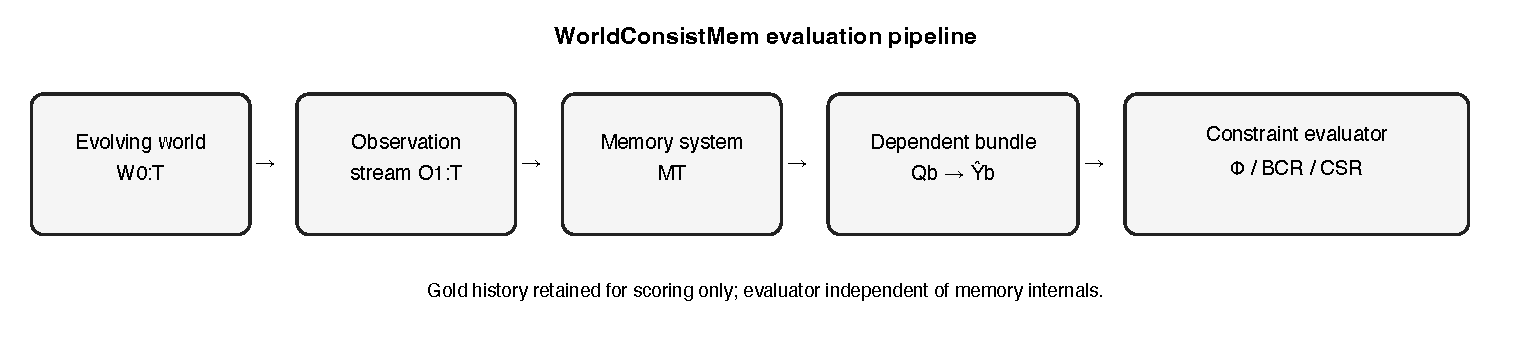
\includegraphics[width=0.92\linewidth]{figures/fig1-pipeline.pdf}
\caption{Evaluation object: evolving world $\rightarrow$ memory $\rightarrow$ dependent bundle $\rightarrow$ joint constraint scoring. Takeaway: BCR scores the answer \emph{set}, not isolated queries.}
\label{fig:pipeline}
\end{figure}

A query bundle $Q_b=\{q_1,\ldots,q_{n_b}\}$ asks interdependent current/historical/transition/relational/provenance/conflict questions about one focal lifecycle. Predictions $\hat Y_b$ come from a reader on $M_T$. Constraints $\mathcal{C}_b$ are compiled from the gold history and query slots. Define the joint consistency predicate
\begin{equation}
\Phi(\hat Y_b;\mathcal{C}_b)=\mathbf{1}\bigl[\forall c\in\mathcal{C}_b:\; c(\hat Y_b)\bigr],
\label{eq:phi}
\end{equation}
with $\Phi=1$ if $\mathcal{C}_b=\emptyset$. Per-query Acc is $\mathrm{Acc}_i=\mathbf{1}[\hat y_i\equiv y_i^*]$ under structured equality. Acc aggregates over queries; $\Phi$ is a property of the full answer set. Neither is a function of the other: high Acc with $\Phi=0$ and low Acc with $\Phi=1$ are both possible (Figure~\ref{fig:inconsistency}; Table~\ref{tab:corruption}).

\begin{figure}[t]
\centering
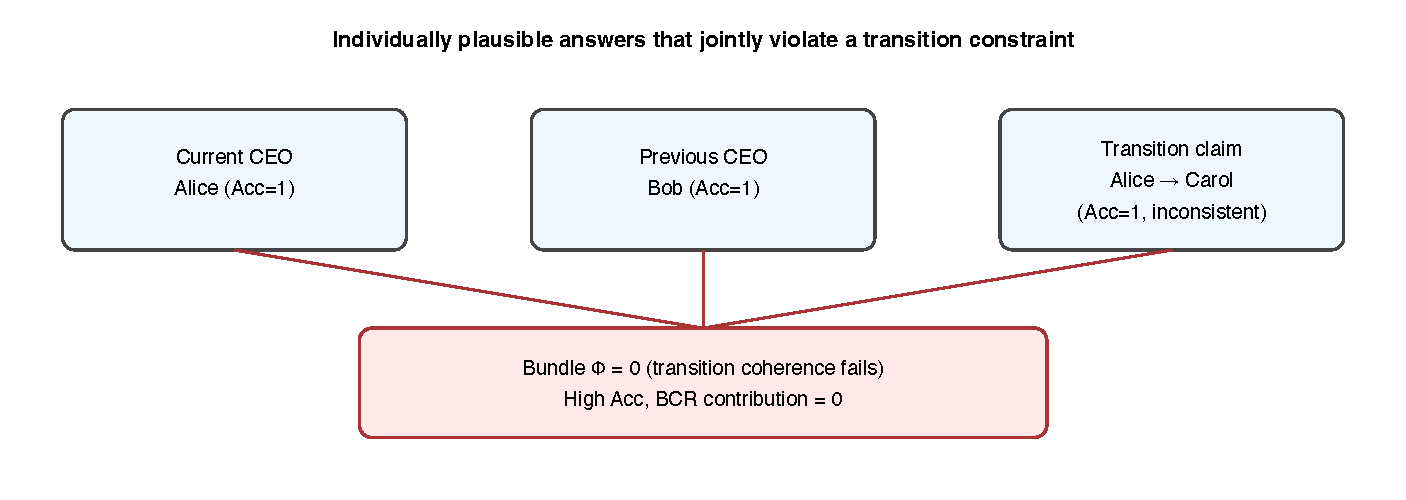
\includegraphics[width=0.88\linewidth]{figures/fig2-inconsistency-example.pdf}
\caption{Central failure mode: individually correct answers with an impossible transition ($\Phi=0$).}
\label{fig:inconsistency}
\end{figure}

This object is for \textbf{memory systems} over evolving worlds, not SMT satisfiability of logical commitments alone~\citep{salla2026crossQueryContradictions,chaudhry2026logicVault}. Any map $O_{1:T}\mapsto M_T$ can be scored with the same $(Q_b,Y_b^*,\mathcal{C}_b)$ protocol.
